% PRISMA 2020 flow diagram (new systematic review; databases + other methods)
% Counts are taken from the stage-wise screening logs in prisma/01-09 of the repository;
% exclusion-reason categories are listed per record in prisma/10_prisma_flow/exclusion_reasons_categorized.csv
\documentclass[border=2pt]{standalone}
\usepackage[T1]{fontenc}
\usepackage{helvet}
\renewcommand{\familydefault}{\sfdefault}
\usepackage{tikz}
\usetikzlibrary{positioning,arrows.meta,calc,fit}
\definecolor{phase}{HTML}{2F5D8A}
\definecolor{phasebg}{HTML}{DCE6F1}
\definecolor{exbg}{HTML}{F4F6F8}
\definecolor{incbg}{HTML}{E3F1E8}
\definecolor{oth}{HTML}{C75B39}
\definecolor{line}{HTML}{39465A}
\begin{document}
\footnotesize\hyphenpenalty=10000\exhyphenpenalty=10000
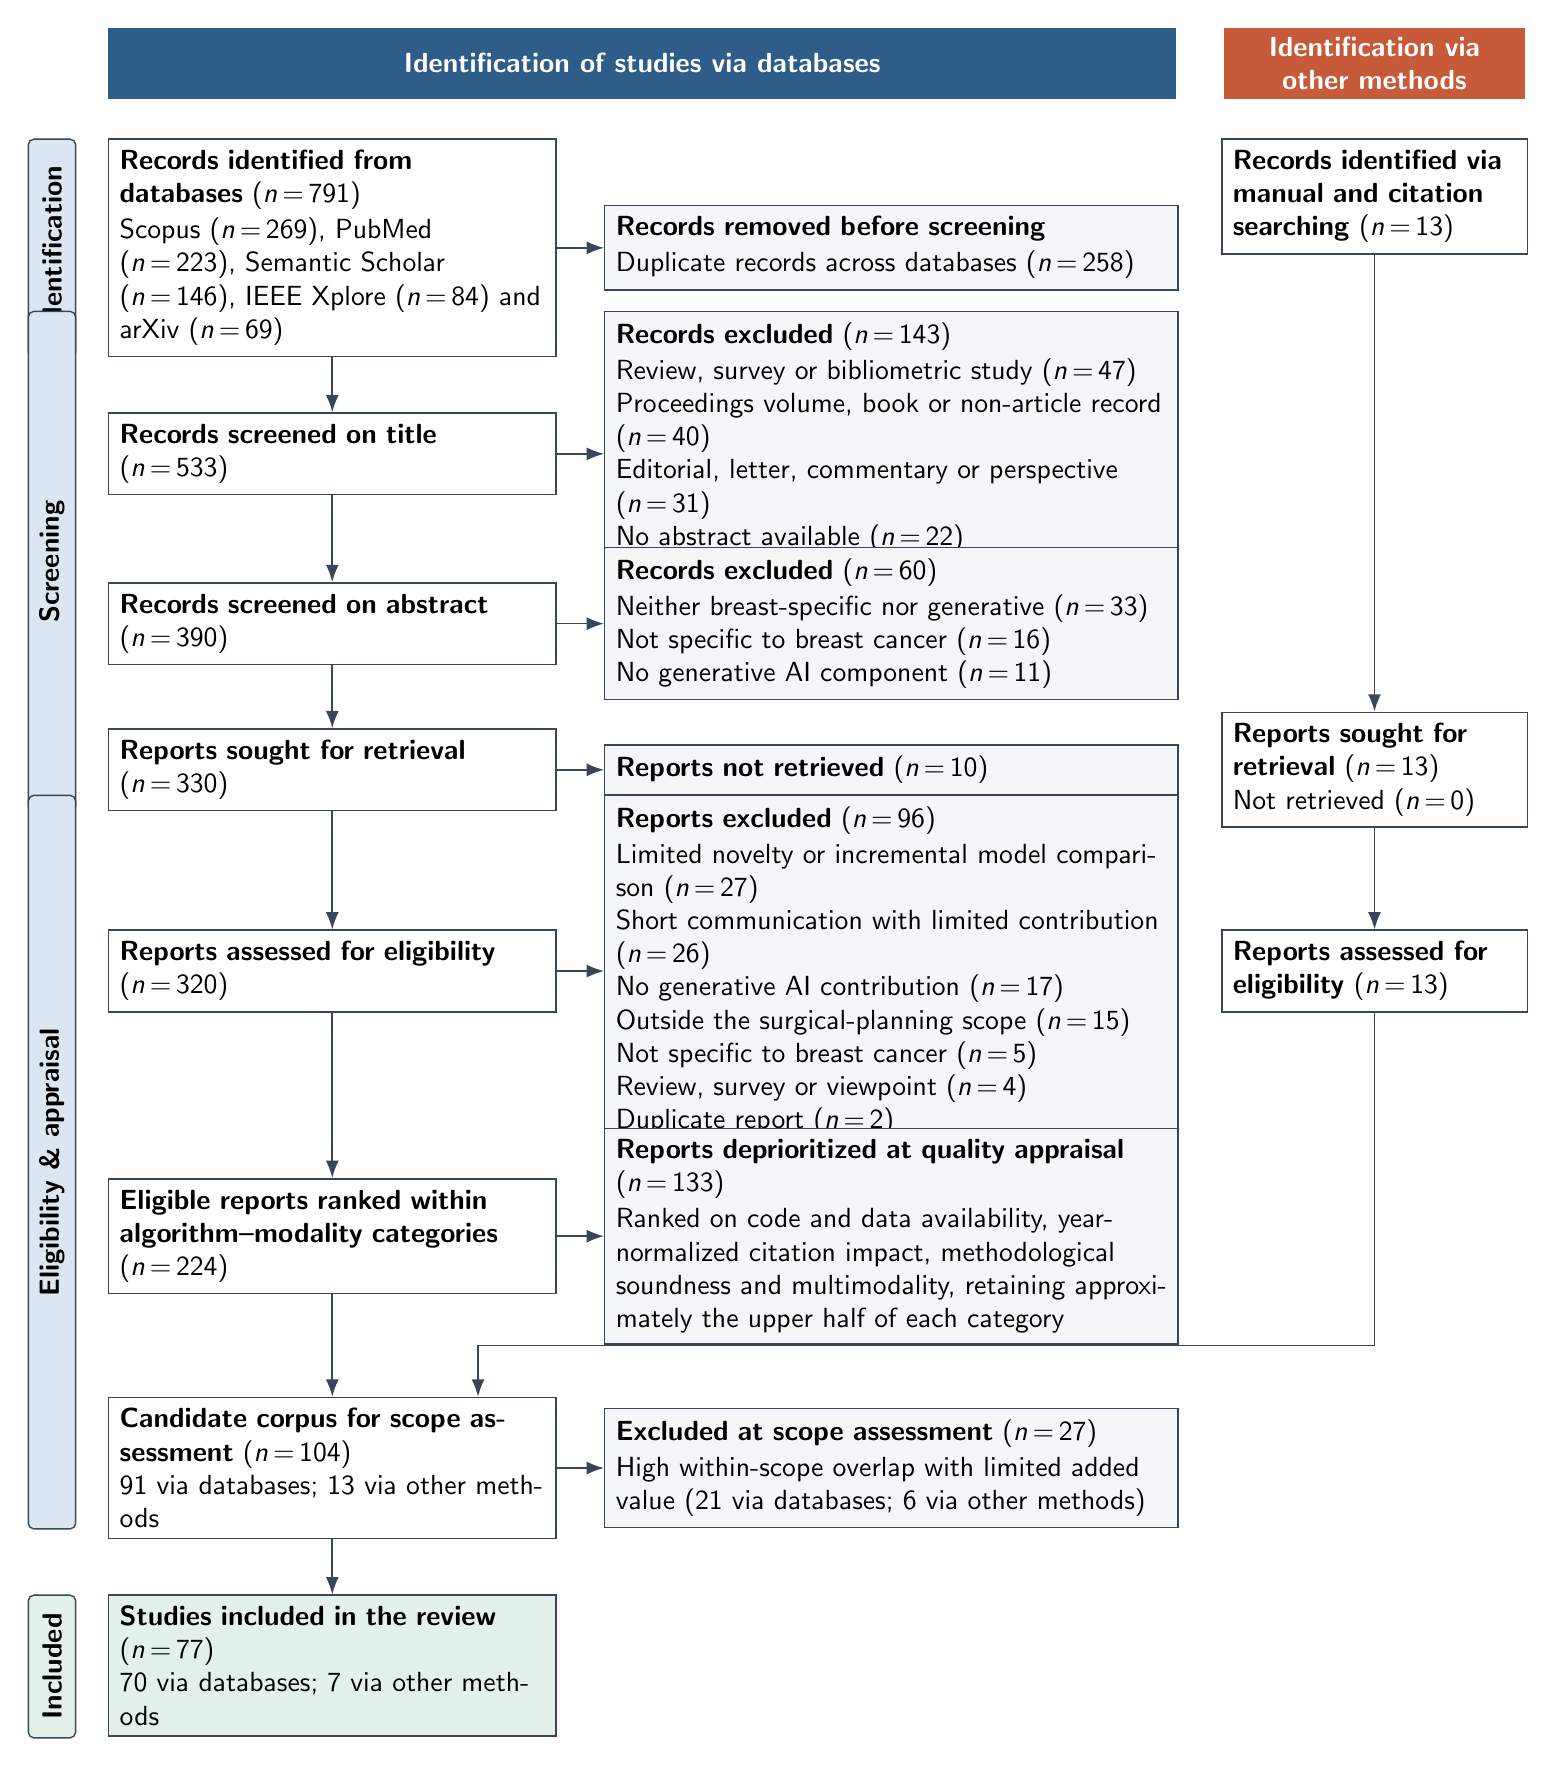
\begin{tikzpicture}[
  node distance=4.2mm and 6mm,
  box/.style={draw=line, line width=0.6pt, fill=white, align=left, text width=#1, inner sep=4pt, minimum height=9mm},
  box/.default=54mm,
  ex/.style={draw=line, line width=0.5pt, fill=exbg, align=left, text width=70mm, inner sep=4pt},
  arr/.style={-{Latex[length=2.2mm]}, line width=0.6pt, draw=line},
  hdr/.style={draw=none, fill=#1, text=white, font=\bfseries, align=center, minimum height=9mm, inner sep=3pt},
]
% ---------------- column headers
\node[hdr=phase, text width=133.5mm] (H1) at (0,0) {Identification of studies via databases};
\node[hdr=oth, text width=36mm, right=6mm of H1] (H2) {Identification via\\ other methods};

% ---------------- identification
\node[box, minimum height=23mm, below=5mm of H1.south west, anchor=north west] (id) {\textbf{Records identified from databases} (\textit{n}\,=\,791)\\[1pt]
Scopus (\textit{n}\,=\,269), PubMed (\textit{n}\,=\,223), Semantic Scholar (\textit{n}\,=\,146), IEEE Xplore (\textit{n}\,=\,84) and arXiv (\textit{n}\,=\,69)};
\node[ex, right=6mm of id] (dup) {\textbf{Records removed before screening}\\[1pt] Duplicate records across databases (\textit{n}\,=\,258)};
\node[box=36mm, below=5mm of H2.south, anchor=north] (oid) {\textbf{Records identified via manual and citation searching} (\textit{n}\,=\,13)};

% ---------------- screening
\node[box, below=7mm of id] (ts) {\textbf{Records screened on title} (\textit{n}\,=\,533)};
\node[ex, right=6mm of ts] (tsx) {\textbf{Records excluded} (\textit{n}\,=\,143)\\[1pt]
Review, survey or bibliometric study (\textit{n}\,=\,47)\\
Proceedings volume, book or non-article record (\textit{n}\,=\,40)\\
Editorial, letter, commentary or perspective (\textit{n}\,=\,31)\\
No abstract available (\textit{n}\,=\,22)\\ Other non-primary record (\textit{n}\,=\,3)};
\node[box, below=11mm of ts] (as) {\textbf{Records screened on abstract} (\textit{n}\,=\,390)};
\node[ex, right=6mm of as] (asx) {\textbf{Records excluded} (\textit{n}\,=\,60)\\[1pt]
Neither breast-specific nor generative (\textit{n}\,=\,33)\\
Not specific to breast cancer (\textit{n}\,=\,16)\\
No generative AI component (\textit{n}\,=\,11)};
\node[box, below=8mm of as] (rs) {\textbf{Reports sought for retrieval} (\textit{n}\,=\,330)};
\node[ex, right=6mm of rs] (rsx) {\textbf{Reports not retrieved} (\textit{n}\,=\,10)};
\node[box=36mm] (ors) at (oid |- rs) {\textbf{Reports sought for retrieval} (\textit{n}\,=\,13)\\ Not retrieved (\textit{n}\,=\,0)};

% ---------------- eligibility and appraisal
\node[box, below=15mm of rs] (el) {\textbf{Reports assessed for eligibility} (\textit{n}\,=\,320)};
\node[ex, right=6mm of el] (elx) {\textbf{Reports excluded} (\textit{n}\,=\,96)\\[1pt]
Limited novelty or incremental model comparison (\textit{n}\,=\,27)\\
Short communication with limited contribution (\textit{n}\,=\,26)\\
No generative AI contribution (\textit{n}\,=\,17)\\
Outside the surgical-planning scope (\textit{n}\,=\,15)\\
Not specific to breast cancer (\textit{n}\,=\,5)\\ Review, survey or viewpoint (\textit{n}\,=\,4)\\ Duplicate report (\textit{n}\,=\,2)};
\node[box, below=21mm of el] (qa) {\textbf{Eligible reports ranked within algorithm--modality categories} (\textit{n}\,=\,224)};
\node[ex, right=6mm of qa] (qax) {\textbf{Reports deprioritized at quality appraisal} (\textit{n}\,=\,133)\\[1pt]
Ranked on code and data availability, year-normalized citation impact, methodological soundness and multimodality, retaining approximately the upper half of each category};
\node[box=36mm] (oel) at (oid |- el) {\textbf{Reports assessed for eligibility} (\textit{n}\,=\,13)};
\node[box, below=13mm of qa] (sc) {\textbf{Candidate corpus for scope assessment} (\textit{n}\,=\,104)\\ 91 via databases; 13 via other methods};
\node[ex, right=6mm of sc] (scx) {\textbf{Excluded at scope assessment} (\textit{n}\,=\,27)\\[1pt]
High within-scope overlap with limited added value (21 via databases; 6 via other methods)};

% ---------------- included
\node[box, fill=incbg, below=7mm of sc, minimum height=11mm] (inc) {\textbf{Studies included in the review} (\textit{n}\,=\,77)\\ 70 via databases; 7 via other methods};

% ---------------- arrows
\foreach \a/\b in {id/ts, ts/as, as/rs, rs/el, el/qa, qa/sc, sc/inc} \draw[arr] (\a) -- (\b);
\foreach \a/\b in {id/dup, ts/tsx, as/asx, rs/rsx, el/elx, qa/qax, sc/scx} \draw[arr] (\a) -- (\b);
\draw[arr] (oid) -- (ors);
\draw[arr] (ors) -- (oel);
\path (qa.south) -- coordinate[pos=0.5] (gap) (sc.north);
\draw[arr] (oel.south) |- ($(gap -| sc.north east)+(-10mm,0)$) -- ($(sc.north east)+(-10mm,0)$);

% ---------------- phase bars
\newcommand{\phasebar}[4]{%
  \path let \p1=(#1), \p2=(#2) in node[draw=line, line width=0.5pt, fill=#4, rounded corners=2pt, minimum width=6mm,
    minimum height={\y1-\y2}, anchor=north east, inner sep=0pt] at ($(id.west |- #1)+(-4mm,0)$) {\rotatebox{90}{\bfseries #3}};}
\phasebar{id.north}{id.south}{Identification}{phasebg}
\phasebar{tsx.north}{rs.south}{Screening}{phasebg}
\phasebar{elx.north}{scx.south}{Eligibility \& appraisal}{phasebg}
\phasebar{inc.north}{inc.south}{Included}{incbg}
\end{tikzpicture}
\end{document}
